% !TeX root = ./0Base.tex

\chapter{Criteria description}

\section{Performance benchmark}

\subsection{Scenarios}\label{sub:scenarios}
The task for each application is to complete simple \acrshort{crud} operations as fast as possible. For comparison of the performance of the applications, a few test cases were developed:

\begin{itemize}
  \item retrieving multiple objects (getMany)
  \item retrieving single object (get)
  \item updating a single object (put)
  \item creating a single object (post)
  \item deleting a single object (delete)
\end{itemize}

They were tested with a few different application loads, which are represented by a number of \acrlong{vu}s (\acrshort{vu}s) - as mentioned in the k6 repository description they are glorified, parallel while(true) loops \cite{k6Git}.
The scenarios chosen for tests are:
\begin{itemize}
  \item 1 \acrshort{vu}
  \item 8 \acrshort{vu}s
  \item 32 \acrshort{vu}s
  \item 128 \acrshort{vu}s
  \item 512 \acrshort{vu}s
\end{itemize}
For a single virtual user case the number of concurrences does not change throughout the duration of the test, however, as suggested in a few articles and k6 documentation, for bigger numbers of concurrent users, it is recommended for the tests to include warmup and cooldown period \cite{whyRampUp} \cite{importanceOfRampUp} \cite{k6LoadTesting}. All tests are 30 seconds long, and tests with more than 1 virtual user include 5 seconds of ramp up time and 5 seconds of ramp down time as shown on figure \ref{fig:vusPerSecond}.

Longer test times did not bring any satisfactory results and only caused CPU throttling problems, thus they were shortened to the period of 30 total seconds, which also made comparison of the results much easier.

Because the results over time were different for each attempt of the test, each test scenario was repeated 3 times. For creation of the graphs presented in chapter \ref{cha:results} for each test average response times were calculated.
\begin{figure}[H]
    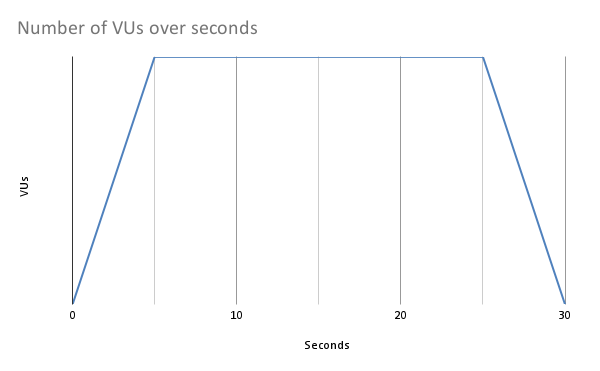
\includegraphics[width=\columnwidth]{figures/pictures/vusPerSecond.png}
    \caption{Amount of VUs per second during the tests}
    \label{fig:vusPerSecond}
\end{figure}


\subsection{Requirements}

To make the results as reliable as possible, a few requirements were introduced. Load tests need to follow the following rules:
\begin{enumerate}
  \item Each scenario must send the same requests to each application.
  \item Before each test the database must be restored to its initial state.
  \item After each test request the response status must be checked for its correctness.
  \item Choice of users for \acrshort{crud} operations must be the same for each application
\end{enumerate}

Applications should be written according to the following requirements:
\begin{enumerate}
  \item Source code and production ready environment should be based on the official documentation whenever that is possible.
  \item Logging and cache must be disabled.
  \item Developer created database model must be the same for each application.
  \item \acrshort{sql} commands generated by applications must return the same results from the prepared database.
  \item Endpoint paths and their arguments must be equal for each application.
  \item Response status and body of each endpoint must be the same for each scenario in each application.
\end{enumerate}

\subsection{Data}\label{sub:population}

For the performance tests some frameworks required initial data to exist in the database (for example PUT endpoint for editing database models), thus at the beginning of the tests for each framework the database is populated. To be sure that the data is consistent, after seeding the database the docker volume that keeps the data is being stored locally, and before each test it is being restored.

\subsection{Application isolation}

To be sure that the applications are running in an isolated environment, docker containers were used. The configuration prepared for the applications included environment preparation (installing necessary packages, providing environment variables), To simplify the research, a Docker Compose configuration was prepared, that builds and starts all the necessary containers at once.

\subsection{Software versions and hardware}

The tests were run on a laptop with the specification presented in table \ref{tab:hardware}.
Frameworks used to build the application were in the versions presented in table \ref{tab:software}.


\FloatBarrier
\begin{table}[!htp]\centering
    \caption{Hardware}\label{tab:hardware}
    \scriptsize
    \begin{tabular}{lrr}\toprule
        Hardware         &                                          \\\midrule
        Processor        & Intel(R) Core(TM) i5-8250U CPU @ 1.60GHz \\
        RAM memory       & 16 GB @ 2400MT/s                         \\
        Operating system & Ubuntu 20.04.2 LTS                       \\
        \bottomrule
    \end{tabular}
\end{table}
\FloatBarrier


\FloatBarrier
\begin{table}[!htp]\centering
    \caption{Frameworks and libraries versions}\label{tab:software}
    \scriptsize
    \begin{tabular}{lrr}\toprule
        Software versions                     &         \\\midrule
        Python                                & 3.1.9   \\
        Django                                & 3.1.4   \\
        Django REST Framework                 & 3.12.2  \\
        gunicorn                              & 20.0.4  \\
        uvicorn                               & 0.13.1  \\\midrule
        C\#                                   & 7.3     \\
        ASP.NET                               & 2.1.1   \\
        Npgsql.EntityFrameworkCore.PostgreSQL & 2.1.1.1 \\\midrule
        Node.js                               & 15.12.0 \\
        Express                               & 4.17.1  \\
        pg-promise                            & 10.9.5  \\
        body-parser                           & 1.19.0  \\
        \bottomrule
    \end{tabular}
\end{table}
\FloatBarrier


\section{Security}
To try to answer the question how secure are the frameworks, three points from \acrshort{owasp} Top 10 API Security vulnerabilities list were chosen. To be precise:
\begin{itemize}
  \item Security Misconfiguration, such as incomplete or unsecure default configurations, permissive \acrshort{cors} or error messages that expose sensitive information,
  \item Injection, such as \acrshort{sql}, NoSQL or Command Injection, where attacker can trick the interpreter into executing unintended commands,
  \item Insufficient Logging \& Monitoring, which extends the time of detecting a breach into the system \cite{owaspTop10}.
\end{itemize}
For security misconfiguration section there will be mentioned common mistakes that can be done when deploying the application and explained harm that can be done when they happen.
Application security will be checked with injection attacks - malicious data will be used to try to exploit the system and return values that should not be available on given path.
The last thing to mention in security part of this thesis will be logging possibilities of the framework.
